\subsection{Process Description}
\label{sec:process}
% Please give a brief update of your food production system’s process (including maintenance and cleaning):
% Fully-detailed process description (incl. setup, operation, maintenance, and cleaning), flow diagram for each
% maximum 5000 characters

\begin{figure}[h!]
    \centering
    \frame{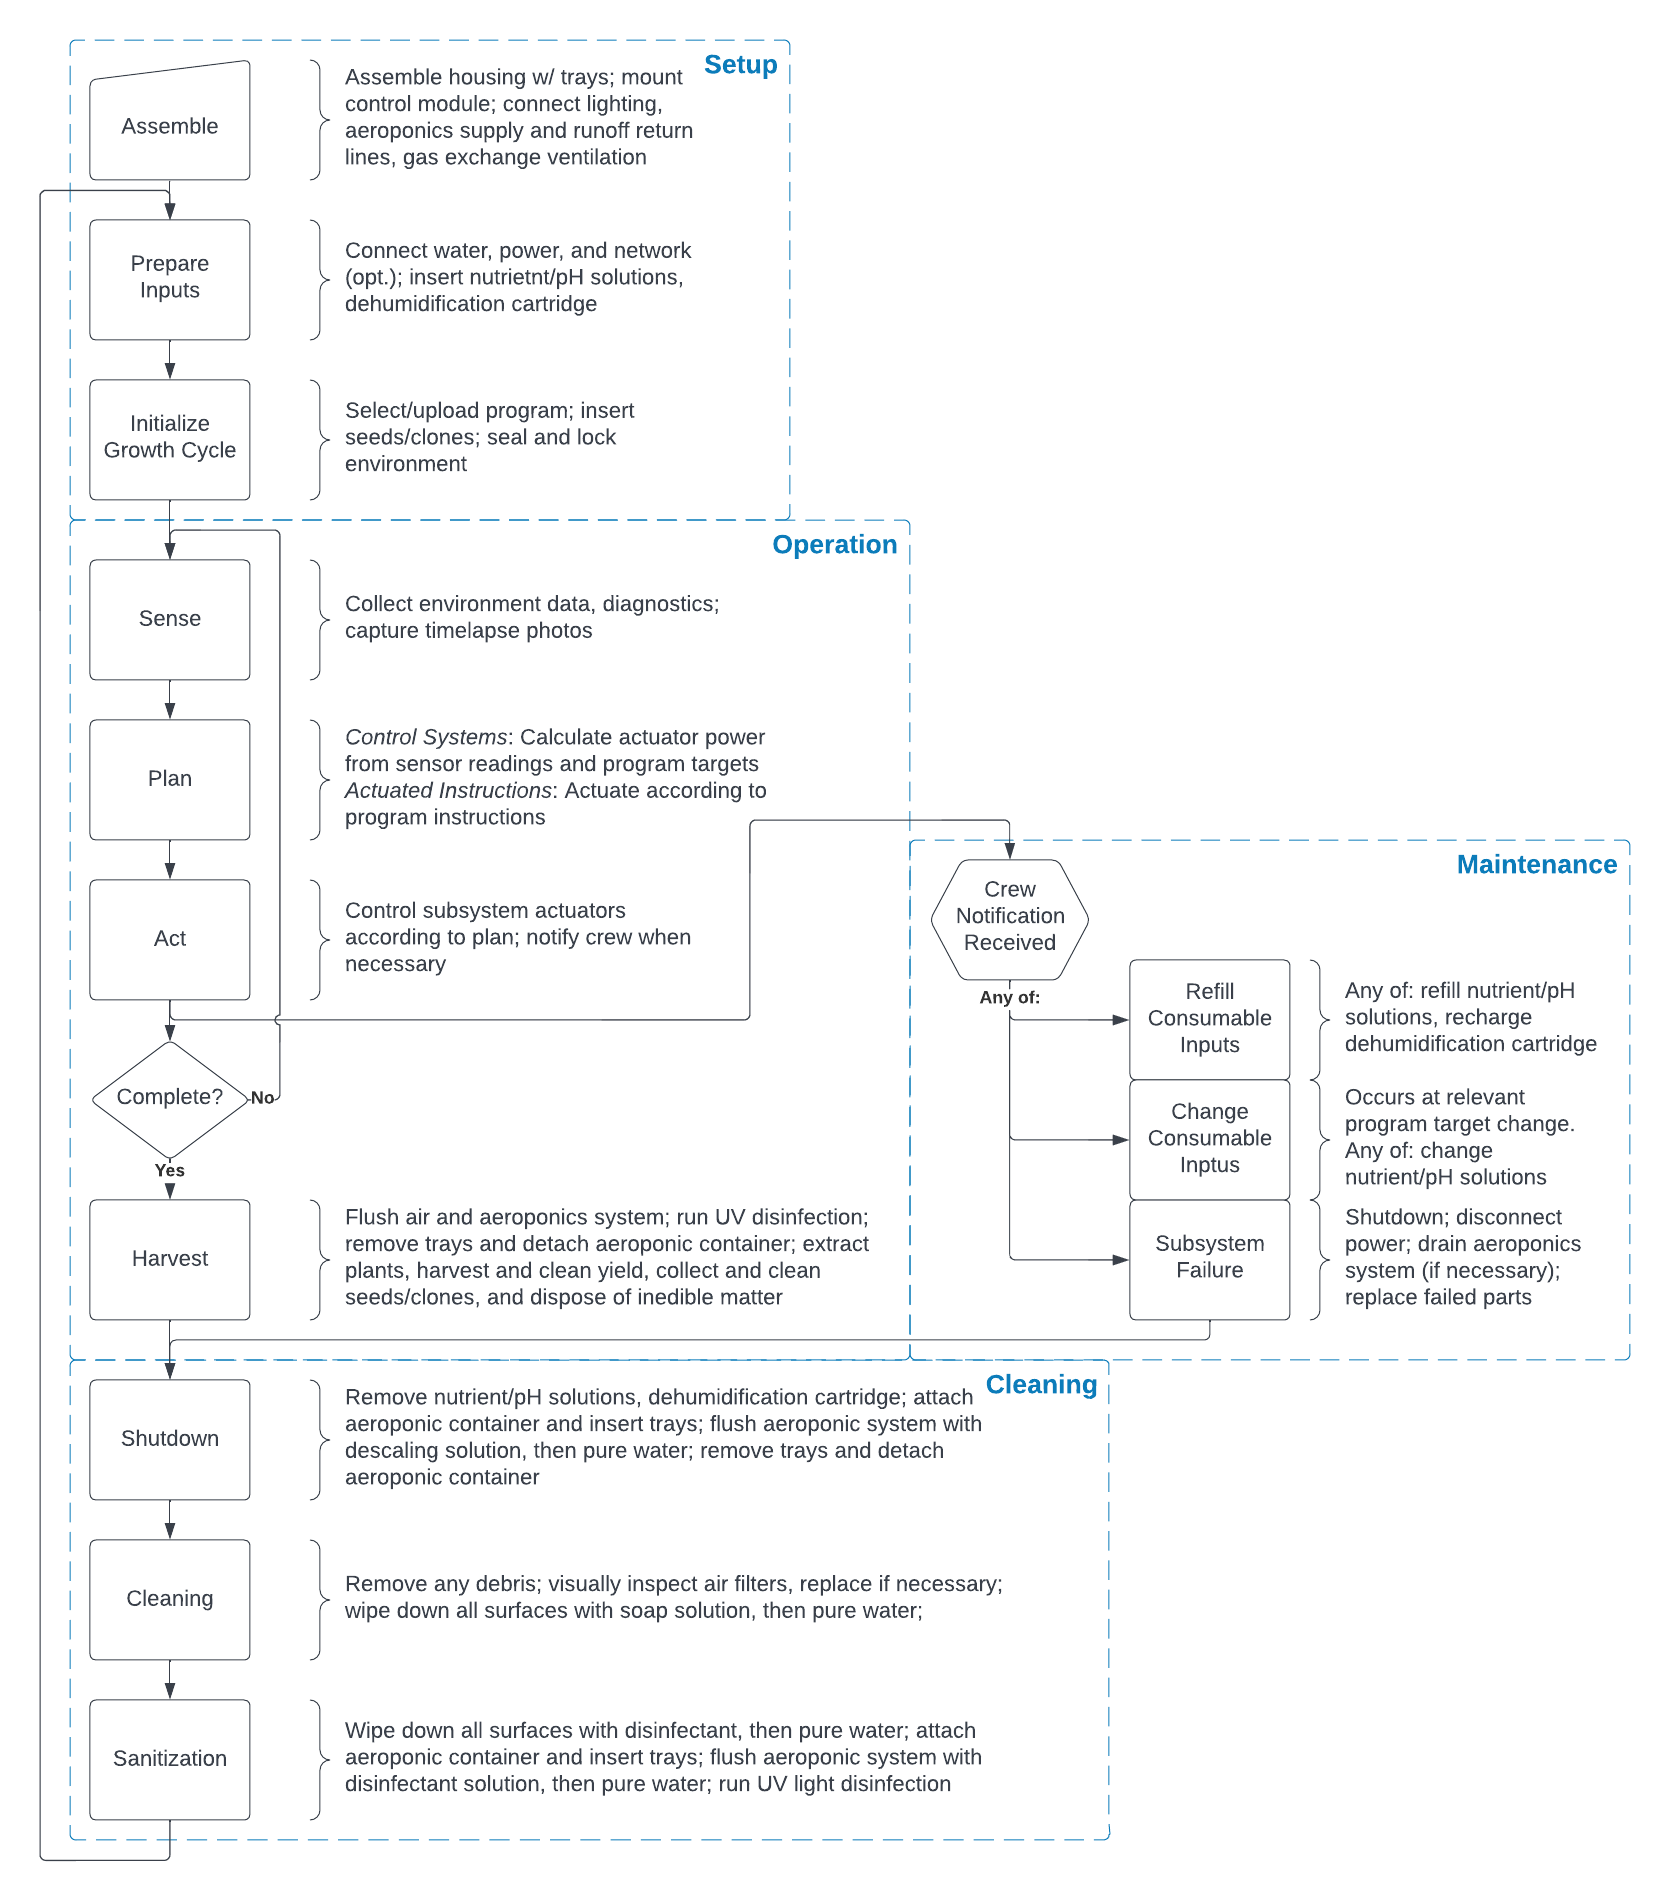
\includegraphics[width=0.85\textwidth]{../assets/figures/process.png}}
    \caption{Process diagram.}
    \label{fig:process}
\end{figure}

\clearpage

\subsubsection{Setup}
\label{sec:process_setup}

\textbf{Assembly}:
\begin{enumerate}
    \item Assemble housing, trays (see \ref{sec:housing});
    \item Mount control module, trays (see \ref{sec:housing});
    \item Connect subsystems to control module:
    \begin{itemize}
        \item \textit{Housing Solenoid Lock}: relay (see \ref{sec:housing})
        \item \textit{Aeroponics Supply \& Runoff Collection Lines}: quick-disconnect (see \ref{sec:aeroponics})
        \item \textit{Lighting Driver Board}: power, control signal (see \ref{sec:lighting})
    \end{itemize}
    \item Connect gas exchange exhaust to ventilation (see \ref{sec:gas});
\end{enumerate}

\textbf{Prepare Inputs}:
\begin{enumerate}
    \item Connect supply inputs:
    \begin{itemize}
        \item \textit{Power}: 120V 60Hz AC (see \ref{sec:automation})
        \item \textit{Network}: ethernet or wireless, optional (see \ref{sec:automation})
        \item \textit{Water}: reverse-osmosis, ambient (see \ref{sec:aeroponics})
    \end{itemize}
    \item Insert consumable inputs:
    \begin{itemize}
        \item \textit{Nutrient/pH Adjusment Solutions}: pouches (see \ref{sec:aeroponics})
        \item \textit{Dehumidification Cartridge}: recharged (see \ref{sec:dehumidification})
    \end{itemize}
\end{enumerate}

\textbf{Initialize Growth Cycle}:
\begin{enumerate}
    \item Select or upload program;
    \item Insert seeds/clones;
    \item Seal and lock environment;
    \item Start growth cycle;
\end{enumerate}

\textbf{Proceed to Operation} (see \ref{sec:process_operation}).

\subsubsection{Operation}
\label{sec:process_operation}

\textbf{Sense, Plan, Act} represents the three simultaneous automatic processes of the program's execution (see \ref{sec:automation}).

\begin{itemize}
    \item \textbf{Sense}: Environment data, diagnostic information, and timelapse photos are captured and stored at regular intervals.
    \item \textbf{Plan}:
    \begin{itemize}
        \item \textit{Control Systems}: Actuator controls are calculated from sensor readings and program targets.
        \item \textit{Actuated Instructions}: Actuator controls are derived from program instructions.
    \end{itemize}
    \item \textbf{Act}: Subsystem actuators are controlled according to plan. Crew is notified to refill consumable inputs when low, change consumable inputs on program target change, and on any subsystem failure (see \ref{sec:process_maintenance}), as well as when to harvest and on End of Program (EoP).
\end{itemize}

\clearpage

\textbf{Harvest and/or EoP}:
\begin{enumerate}
    \item Exhaust all air (automatic, see \ref{sec:gas});
    \item Flush aeroponics system with pure water (automatic, see \ref{sec:aeroponics});
    \item Run UV disinfection (automatic, see \ref{sec:lighting});
    \item Unlock and open environment;
    \item Remove trays (see \ref{sec:housing}) and detach aeroponic container (see \ref{sec:aeroponics});
    \item \textbf{If EoP}: Extract plants;
    \item Harvest and clean yield;
    \item Collect, clean, and store seeds/clones;
    \item \textbf{If EoP}: Dispose of inedible matter;
\end{enumerate}

\textbf{If EoP, proceed to Cleaning} (see \ref{sec:process_cleaning})\textbf{. Otherwise, seal and lock environment and resume program.}

\subsubsection{Maintenance}
\label{sec:process_maintenance}

\textbf{Notification Handling}:
\begin{itemize}
    \item \textit{Refill Consumable Inputs}: includes refilling nutrient/pH adjustment solutions (see \ref{sec:aeroponics}), recharging the dehumidification cartridge (see \ref{sec:dehumidification})
    \item \textit{Change Consumable Inputs}: includes changing nutrient/pH adjustment solutions (see \ref{sec:aeroponics})
    \item \textit{Subsystem Failure}: all operation stopped, proceed to \textit{Shutdown} (see \ref{sec:process_cleaning}), disconnect power (see \ref{sec:automation}), then drain aeroponics system if necessary (see \ref{sec:aeroponics}) and replace failed components
\end{itemize}

\subsubsection{Cleaning}
\label{sec:process_cleaning}

\textbf{Shutdown}:
\begin{enumerate}
    \item Remove nutrient/pH solutions (see \ref{sec:aeroponics}), dehumidification cartridge (see \ref{sec:dehumidification});
    \item Attach aeroponic container (see \ref{sec:aeroponics}) and insert trays (see \ref{sec:housing});
    \item Flush aeroponic system with descaling solution (see \ref{sec:aeroponics});
    \item Flush aeroponic system with pure water (see \ref{sec:aeroponics});
    \item Remove trays (see \ref{sec:housing}) and detach aeroponic container (see \ref{sec:aeroponics});
\end{enumerate}

\textbf{Cleaning}:
\begin{enumerate}
    \item Visually inspect all surfaces for debris (remove) and components for damage (replace);
    \item Visually inspect all air filters (see \ref{sec:dehumidification}, \ref{sec:gas}), replace if necessary;
    \item Wipe down all surfaces with soap solution;
    \item Wipe down all surfaces with pure water;
\end{enumerate}

\textbf{Sanitization}:
\begin{enumerate}
    \item Wipe down all surfaces with disinfectant solution;
    \item Wipe down all surfaces with pure water;
    \item Dry all surfaces;
    \item Attach aeroponic container (see \ref{sec:aeroponics}) and insert trays (see \ref{sec:housing});
    \item Flush aeroponic system with disinfectant solution (see \ref{sec:aeroponics});
    \item Flush aeroponic system with pure water (see \ref{sec:aeroponics});
    \item Seal and lock environment;
    \item Run UV sanitization (\ref{sec:lighting});
\end{enumerate}

\textbf{Proceed to Prepare Inputs} (see \ref{sec:process_setup}).